\section{Experiments, independent checks, and practical effect}
\label{sec:experiments}

The experiments test mathematical conventions, certificate soundness,
integration behavior, and the performance of particular workloads.
They do not establish an asymptotic upper bound. All example sources,
plain PD fixtures, complete certificates, seeds, commands, and raw
timing samples are included in the archive.

\subsection{Validation layers}

The unchanged pinned baseline passes 134 test methods. The final integrated
suite passes 152 methods, including twelve new arithmetic methods and
six new local-pattern methods. The final full-suite run took 30.415 seconds
as reported by \code{unittest}, with measured process wall time
30.651362 seconds and exit code zero. The baseline and integrated logs
are kept separately, so an old documentation count does not obscure the
actual test coverage.

The new tests exercise 76 small rational closures and 56 small two-tangle
closures against an independently constructed scalar Khovanov cube;
160 random Montesinos examples are checked against exact Alexander
determinants. They also cover a small complete identity matrix,
determinant-one knots with exceptional orders \((2,3,5)\) and
\((2,3,7)\), negative and zero coefficients, intermediate infinity,
final-infinity rejection, mirror and pickle behavior, mutation and
certificate corruption, expansion ceilings, large integer coefficients,
and local occurrence invariance.

Three further diagnostics are independent of the production arithmetic
decision:
\begin{enumerate}
\item The identity-family script verifies all
\(\sum_{m=0}^{10}4^m=1{,}398{,}101\) entries through \(m=10\).
The largest matrix is \(1024\times1024\). It checks primitivity, parity,
diagonal determinants, the stronger off-diagonal gap, and a separately
implemented twist/rotation program. The topological assertion is supplied
by Theorem~\ref{thm:rational-boolean-identity}, not by these finite checks.
\item The independent Montesinos audit evaluates 1,200 sources: 718
one-component constructed PDs against exact Alexander determinants and
482 link cases against actual component counts. It also performs 1,436
mirror/pickle roundtrip checks and verifies the reinitialization guard.
\item The independent local audit rejects twelve forged certificate
variants, invalidates a witness after a selected crossing switch,
checks forty combinations of crossing reordering, relabeling,
half-turns, and mirroring, and finds no false rejection on 31 known
identity-family unknots. It also verifies a three-exceptional local
occurrence and rejects patterns that are unknottable, integral, or have
an internal closed component.
\end{enumerate}

The checkpoint diagnostic constructs 21 actual diagrams, for \(0\le k\le20\),
checks the two continued fractions and exact counts \(8k+4\), and verifies
their arithmetic unknot certificates. For the small prefix closures it
also performs fourteen independent numerator/denominator Alexander checks
and six independent scalar-cube rank checks. It checks the ordinary
ungraded and strengthened graded lower-bound formulas separately.

Finally, the integration patch was applied to an isolated exact baseline.
All 81 resulting noncache files matched the delivered \code{fast}
snapshot byte for byte. The eighteen new test methods passed there with
\code{PYTHONPATH} removed and no dependence on the outer experiment
directory. This checks that the proposed repository integration is
self-contained. It does not certify a proof-assistant formalization.

\subsection{Timing protocol and comparison scope}

The recorded environment is Python 3.12.14 on x86-64 Linux. The benchmark
uses a warm in-process interpreter, seven paired rounds per case, a
three-second budget, and a 20,000-object complex ceiling. Every timed
recognition call receives a freshly constructed and validated diagram,
so neither branch benefits from previously populated geometry caches.

For each structured case a round executes the old path \(A\), five samples
of the new path \(B\), and \(A\) again. The round's baseline is the mean
of the two \(A\) times; its new time is the median of the five \(B\) samples.
Reported times are medians across rounds, and reported speedups are
medians of the seven paired ratios. Thus the ratio of the two separately
reported medians need not equal the reported paired speedup.

The old path is the updated code with \code{use_rational=False}, on the
same expanded PD as the enabled path. It measures the effect of the added
stage without changing the topology or input ordering. Recognition-stage
timing excludes construction for both paths. A separate column times
new PD construction plus recognition. No claim about CLI startup, disk
I/O, or deployment latency is drawn from these numbers.

A baseline \unknown\ result is censored. Its elapsed time is time to
the cap, not a completed solve, so it receives no speedup ratio.
Local-pattern cases use the sequence \(A,B,A\) on fresh plain PDs;
their wrapper searches before falling back. That deliberately exposes
search overhead on cases already decided cheaply by existing filters.

\subsection{Rational-pair unknots}

Use \(w=(AB)^k\), so \(m=2k\) and the displayed unknot has \(n=4m+4\)
crossings. Table~\ref{tab:rational-benchmarks} gives the measured results.
The new method is the complete two-bridge determinant branch on these
supplied sources.

\begin{table}[htbp]
\centering\small
\begin{tabular}{rrrrrr}
\toprule
\(n\) & Old recognition (ms) & New recognition (\(\mu\)s) &
New total (ms) & Paired speedup & Old status\\
\midrule
12 & 3.068 & 19.79 & 0.129 & \(147.9\times\) & \unk\\
20 & 5.707 & 22.28 & 0.263 & \(253.2\times\) & \unk\\
28 & 14.926 & 23.58 & 0.226 & \(610.9\times\) & \unk\\
36 & 56.906 & 25.48 & 0.272 & \(1997.1\times\) & \unk\\
44 & 66.522* & 30.23 & 0.327 & --- & \unknown\\
52 & 78.735* & 30.04 & 0.381 & --- & \unknown\\
\bottomrule
\end{tabular}
\caption{Fresh-diagram recognition measurements. \emph{New total} includes
PD construction. Asterisks mark time to an object cap, not a completed
baseline decision. Ratios are paired medians.}
\label{tab:rational-benchmarks}
\end{table}

The most substantial comparisons are the completed diagonal unknot cases:
all ordinary one-sided invariant filters are inconclusive, and the old path
reaches the exact Khovanov scan. At 44 and 52 crossings, the new arithmetic
branch completes while the explicit old path reaches the object ceiling.
This is an improvement in achieved decisions at a fixed budget, not a
quantified speedup over an unknown eventual completion time.

The post-elimination object counts in the completed old scans are
\[
10,\quad58,\quad338,\quad1970.
\]
Their maximum boundary has only four endpoints. For \(k=1,2,3,4\), these
counts equal \(p_k+q_k\), the graded lower bound in
Corollary~\ref{cor:graded-checkpoint-size}. The corresponding counts before
elimination are \(27,157,915,5333\). The numerical agreement supports the
interpretation that the retained information itself is costly, rather
than merely reflecting missed elementary cancellations. It is not a proof
that every later scan is minimal, nor a lower bound for every scan order.

For perspective, at \(k=12\), the mathematical family has a displayed
100-crossing unknot and
\[
 p_{12}+q_{12}=2{,}623{,}476{,}242.
\]
A full graded complex at that prefix has at least this many explicit
summands. This number is a theorem-derived lower bound, verified
arithmetically by the diagnostic, not a claim that a billion-object
benchmark was run.

\subsection{Nontrivial sources and compressed coefficients}

The off-diagonal example uses \(u=A^8\) and \(w=B^8\). Its 36-crossing
knot is already rejected by the baseline Rasmussen interval in a median
0.102 ms. The arithmetic stage takes 17.64 \(\mu\)s, with paired
speedup \(5.35\times\); its construction-plus-recognition time is
0.243 ms. This is a useful guard against interpreting every rational
example as an exponential fallback case.

Table~\ref{tab:pretzel-benchmarks} uses the Alexander-one family
\eqref{eq:mon:family}. These knots pass the determinant and Alexander-one
tests by construction; the baseline rejects them with its Jones filter.
Their arithmetic nontriviality follows from three exceptional fibers.

\begin{table}[htbp]
\centering\small
\begin{tabular}{rrrrrr}
\toprule
\(a\) & Crossings & Old recognition (ms) & New recognition (\(\mu\)s) &
New total (ms) & Paired speedup\\
\midrule
3 & 15 & 0.964 & 20.44 & 0.148 & \(46.0\times\)\\
7 & 47 & 3.318 & 22.11 & 0.311 & \(166.1\times\)\\
31 & 575 & 35.322 & 40.14 & 4.973 & \(977.9\times\)\\
\bottomrule
\end{tabular}
\caption{Alexander-one, signature-zero, nontrivial Montesinos knots.
The large recognition-only ratios exclude source expansion from both
recognition timers; the end-to-end column makes that cost visible.}
\label{tab:pretzel-benchmarks}
\end{table}

A separate compressed experiment chooses \(a=2^b+1\), using
\[b\in\{64,256,1024,4096,16384,65536\},\]
and calls the arithmetic API
without constructing any PD. The resulting certificates all have
determinant one and reject via the exceptional-fiber argument.
For the last sample, \(a\) has 65,537 bits, the expanded crossing count
has 131,072 bits, and the median production-certificate time is
1.383 ms. Its maximum tracked arithmetic entry length is 262,144 bits.
The certificate verifier is checked outside that production timer.
These numbers illustrate the difference between compressed and expanded
input models; they do not represent the processing of an explicitly
listed diagram with that many crossings.

\subsection{Local search: useful certificates, mixed performance}

Table~\ref{tab:local-benchmarks} records the wrapper that searches first.
The first three rows are negative controls for the default six-template
catalogue. The last two replace a crossing disk in the Conway PD by an
actual forbidden tangle, producing 16- and 25-crossing host diagrams.
Those two rows use the supplied relevant template, so they should not
be compared to an exhaustive template-discovery procedure.

\begin{table}[htbp]
\centering\small
\begin{tabularx}{\textwidth}{X r r r r}
\toprule
Case & \(n\) & Old (ms) & Wrapper (ms) & Paired speedup\\
\midrule
Conway catalogue control & 11 & 0.706 & 1.197 & \(0.59\times\)\\
Hard-unknot catalogue control & 8 & 0.444 & 0.691 & \(0.64\times\)\\
Trefoil catalogue control & 3 & 0.015 & 0.065 & \(0.26\times\)\\
Planted \(1/3+1/3\) & 16 & 0.320 & 0.276 & \(1.21\times\)\\
Planted \(1/(-3)+1/5+1/7\) & 25 & 0.049 & 0.328 & \(0.15\times\)\\
\bottomrule
\end{tabularx}
\caption{Local witness discovery is sound but not a universal speed
improvement. A ratio below one means the wrapper is slower. The cheap
Rasmussen interval already rejects the last host, explaining its regression.}
\label{tab:local-benchmarks}
\end{table}

The local certificate is mathematically stronger than merely checking one
chosen closure, but that does not make its current placement optimal.
Searching before a cheap Seifert or Rasmussen certificate can lose time.
The appropriate current release policy is optional search, with future
experiments on placement after cheap filters and before expensive scans.
The modest planted two-summand improvement should not be overinterpreted:
submillisecond timings are noisy, the sample is small, and the control
ratios already expose nontrivial variation.

\IfFileExists{figures/benchmarks.png}{
\begin{figure}[htbp]
\centering
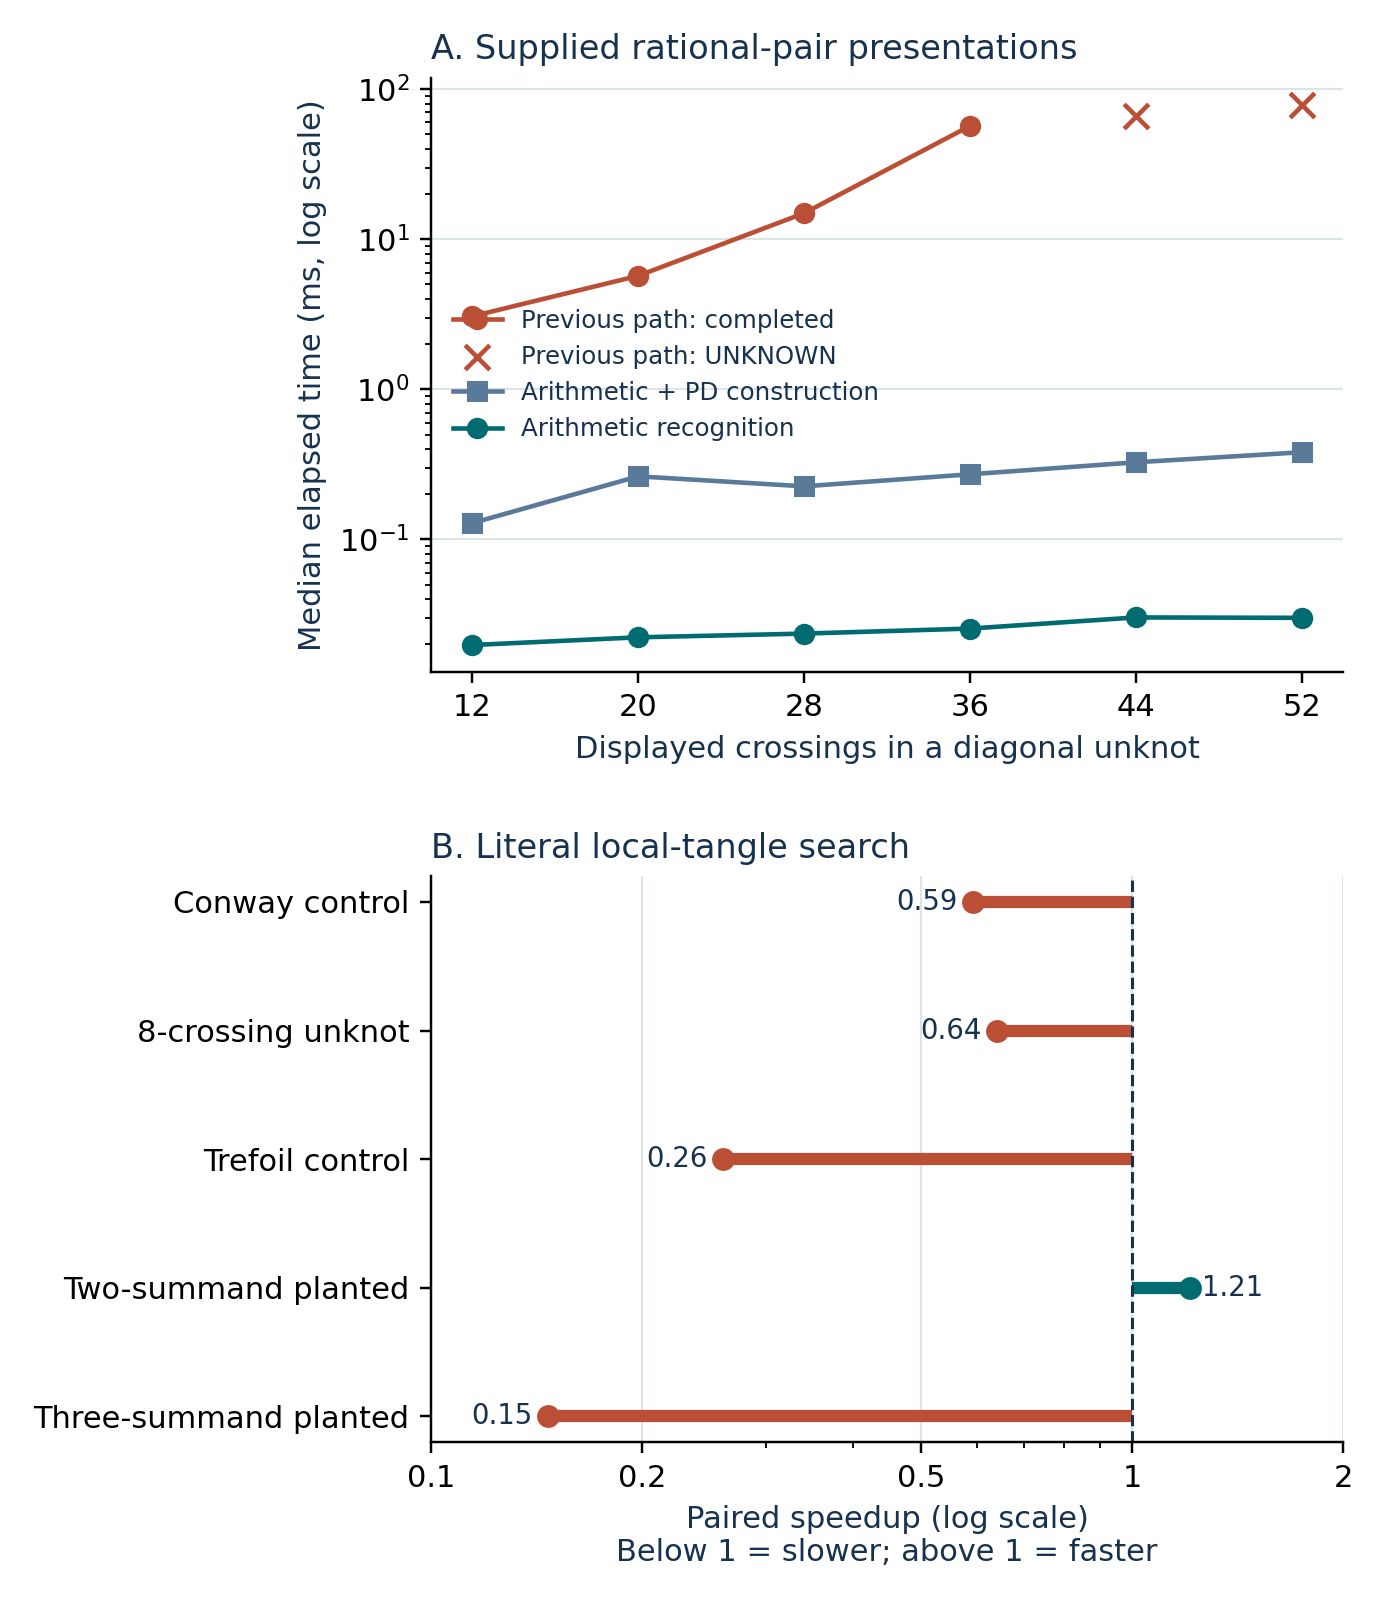
\includegraphics[width=\textwidth]{figures/benchmarks.png}
\caption{Recorded pipeline behavior. Top: diagonal unknot times, with
baseline cap exits marked separately from completed decisions. Bottom:
the optional local wrapper's paired speedups, including all measured
regressions. The figure is generated from the supplied JSON, not fitted
to an asymptotic model.}
\label{fig:benchmarks}
\end{figure}
}{}

\subsection{Reproducibility limits and useful follow-up measurements}

The archive's benchmark driver records every timing sample, both baseline
result objects and one new-path result per structured round. Local rounds
retain all three result objects. Recorded evidence includes methods, available
scan statistics, and the baseline before/after control ratio; end-to-end
and compressed calls retain their timing samples and stated summaries. It can regenerate the source examples and
planted PDs. The plotting script reads the recorded JSON and requires no
new timing run. A separate reproducibility driver exposes the quick tests,
full suite, mathematical diagnostics, and optional repeated benchmarks.

The measurements establish performance for these sources and this
environment. They do not establish average-case behavior on random knots,
the effectiveness of discovering hidden Montesinos structure, or the
maximum performance of every pre-existing backend. In particular, the
primary ablation compares the new arithmetic branch to the default
previous path, not to a competition among all backend settings.
The useful next comparisons are plain-PD rational extraction, pipeline
placement of local search, stronger adversarial source scrambling,
independent environments, and accounting for expanded diagram construction.
The mathematical quadratic arithmetic bound rests on the proof above,
not on fitting the six compressed timing points.
